%%%%%%%%%%%%%%%%%%%%%%%%%%%%%%%%%%%%%%%%%%%%%%%%%%%%%%%%%%%%%%%%%%%%%%%%%%%%%%%%%%
\begin{frame}[fragile]\frametitle{}
\begin{center}
{\Large Exploratory Data Analysis}
\end{center}
\end{frame}

%%%%%%%%%%%%%%%%%%%%%%%%%%%%%%%%%%%%%%%%%%%%%%%%%%%%%%%%%%
\begin{frame}[fragile]\frametitle{Data Exploration}	
Data Exploration: a preliminary investigation of the data in order to better understand its specific characteristics
\end{frame}

%%%%%%%%%%%%%%%%%%%%%%%%%%%%%%%%%%%%%%%%%%%%%%%%%%%%%%%%%%
\begin{frame}[fragile]\frametitle{Data Exploration}	
\begin{itemize}
\item Machine Learning won't accept ANY data that you supply.
\item Garbage In - Garbage Out
\item If you are struggling with model accuracy, then data exploration techniques will come to your rescue.
\end{itemize}
\end{frame}



%%%%%%%%%%%%%%%%%%%%%%%%%%%%%%%%%%%%%%%%%%%%%%%%%%%%%%%%%%
\begin{frame}[fragile]\frametitle{Exploring Data Analysis - EDA}	
\begin{itemize}
\item Patterns can sometime be found simply by visualizing the data
\item Summary statistics also used
\item Most summary statistics can be calculated in a single pass through the data
\end{itemize}
\end{frame}

%%%%%%%%%%%%%%%%%%%%%%%%%%%%%%%%%%%%%%%%%%%%%%%%%%%%%%%%%%
\begin{frame}[fragile]\frametitle{Exploring Data Analysis - EDA}	
Steps to  understand, clean and prepare your data for building your 
predictive model: 

\begin{itemize}
\item Variable Identification 
\item Univariate Analysis 
\item Bi-variate Analysis 
\item Missing values treatment 
\item Outlier treatment 
\item Variable transformation 
\item Variable creation 
\end{itemize}
\end{frame}

%%%%% A Comprehensive Guide to Data Exploration Business Analytics  - Sunil Ray , January 10, 2016 / 27  


%%%%%%%%%%%%%%%%%%%%%%%%%%%%%%%%%%%%%%%%%%%%%%%%%%%%%%%%%%
\begin{frame}[fragile]\frametitle{Variable Identification }	
\begin{itemize}
\item Identify Predictor (Input) and Target (output) variables.
\item Identify the data type and category of the variables. 
\end{itemize}
\end{frame}


%%%%%%%%%%%%%%%%%%%%%%%%%%%%%%%%%%%%%%%%%%%%%%%%%%%%%%%%%%
\begin{frame}[fragile]\frametitle{Variable Identification }	
Example:- Suppose, we want to predict, whether the students will play cricket or not (refer 
below data set).

\begin{center}
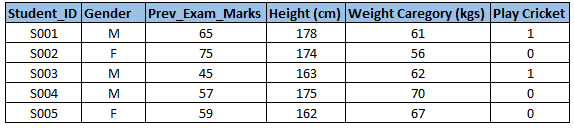
\includegraphics[width=\linewidth,keepaspectratio]{eda1}
\end{center}

Here you need to identify:
\begin{itemize}
\item  Predictor variables
\item Target variable
\item Data type of variables 
\item Category  of  variables.
\end{itemize}
\end{frame}

%%%%%%%%%%%%%%%%%%%%%%%%%%%%%%%%%%%%%%%%%%%%%%%%%%%%%%%%%%
\begin{frame}[fragile]\frametitle{Variable Identification }	
\begin{center}
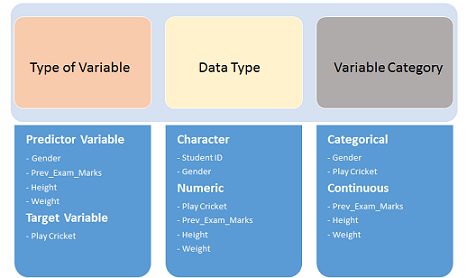
\includegraphics[width=\linewidth,keepaspectratio]{eda2}
\end{center}
\end{frame}


%%%%%%%%%%%%%%%%%%%%%%%%%%%%%%%%%%%%%%%%%%%%%%%%%%%%%%%%%%
\begin{frame}[fragile]\frametitle{Uni-variate Analysis}	
\begin{itemize}
\item  Explore variables one by one
\item Method of analysis depends on type: categorical or continuous
\item Also used to highlight missing and outlier values
\end{itemize}
\end{frame}

%%%%%%%%%%%%%%%%%%%%%%%%%%%%%%%%%%%%%%%%%%%%%%%%%%%%%%%%%%
\begin{frame}[fragile]\frametitle{Univariate Analysis}	
Categorical:   use frequency table to understand distribution of each category.
%	\begin{itemize}
%	\item Examine the mode, 2nd mode, mode \%, and 2nd mode \%
%	\item Represent the most common levels within these features
%	\item Will identify if any levels dominate the dataset. 
%	\end{itemize}
\end{frame}

%%%%%%%%%%%%%%%%%%%%%%%%%%%%%%%%%%%%%%%%%%%%%%%%%%%%%%%%%%
\begin{frame}[fragile]\frametitle{Uni-variate Analysis}	
Continuous:  understand the central tendency  and  spread  of  the  variable. 
	\begin{itemize}
	\item Examine the mean and standard deviation of each feature
	\item Get a sense of the central tendency and variation of the values
	\item Examine the minimum and maximum values to understand the range that is possible for each feature
	\item Histograms of continuous features will resemble the following well understood shapes (probability distributions)
	\item Recognizing the distribution of values for a feature will be useful when applying machine learning models
	\end{itemize}	
\end{frame}



%%%%%%%%%%%%%%%%%%%%%%%%%%%%%%%%%%%%%%%%%%%%%%%%%%%%%%%%%%%
%\begin{frame}[fragile]\frametitle{Univariate Analysis}	
%\begin{center}
%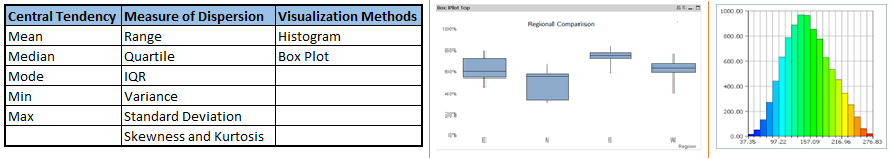
\includegraphics[width=\linewidth,keepaspectratio]{eda3}
%\end{center}
%So, descriptive statistics.
%\end{frame}
%
%%%%%%%%%%%%%%%%%%%%%%%%%%%%%%%%%%%%%%%%%%%%%%%%%%%%
%\begin{frame}[fragile] \frametitle{Uniform Distribution}
%\adjustbox{valign=t}{
%\begin{minipage}{0.45\linewidth}
%\begin{center}
%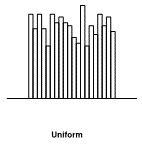
\includegraphics[width=0.8\linewidth,keepaspectratio]{unidist}
%\end{center}
%\end{minipage}
%}
%\hfill
%\adjustbox{valign=t}{
%\begin{minipage}{0.45\linewidth}
%\begin{itemize}
%\item A uniform distribution indicates that a feature is equally likely to take a value in any of the ranges present. 
%\item Sometimes indicative of a feature such as an ID, rather than something more interesting
%\end{itemize}
%\end{minipage}
%}
%\end{frame}


%%%%%%%%%%%%%%%%%%%%%%%%%%%%%%%%%%%%%%%%%%%%%%%%%%%%
%\begin{frame}[fragile] \frametitle{Normal Distribution}
%\adjustbox{valign=t}{
%\begin{minipage}{0.45\linewidth}
%\begin{center}
%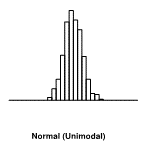
\includegraphics[width=0.8\linewidth,keepaspectratio]{normdist}
%\end{center}
%\end{minipage}
%}
%\hfill
%\adjustbox{valign=t}{
%\begin{minipage}{0.45\linewidth}
%\begin{itemize}
%\item Naturally occurring phenomena (heights, weights of a randomly selected group of men, women) tend to follow a normal distribution.
%\item Features following a normal distribution are characterized by a strong tendency towards a central value and symmetrical variation to either side of this. 
%\item Unimodal: single peak around the central tendency
%\end{itemize}
%\end{minipage}
%}
%\end{frame}
%

%%%%%%%%%%%%%%%%%%%%%%%%%%%%%%%%%%%%%%%%%%%%%%%%%%%
\begin{frame}[fragile] \frametitle{Normal Distribution}
\begin{center}
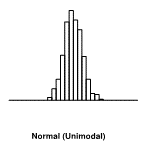
\includegraphics[width=0.3\linewidth,keepaspectratio]{normdist}
\end{center}
\begin{itemize}
\item Naturally occurring phenomena (heights, weights of a randomly selected group of men, women) tend to follow a normal distribution.
\item Features following a normal distribution are characterized by a strong tendency towards a central value and symmetrical variation to either side of this. 
%\item Unimodal: single peak around the central tendency
\end{itemize}
\end{frame}


%%%%%%%%%%%%%%%%%%%%%%%%%%%%%%%%%%%%%%%%%%%%%%%%%%%
\begin{frame}[fragile] \frametitle{68-95-99.7 Rule}
\begin{itemize}
\item The 68 - 95 - 99.7 rule is a useful characteristic of the normal distribution.
\item The rule states that approximately: 
	\begin{itemize}
	\item 68\% of the observations will be within one $sigma$ of $\mu$ 
	\item 95\% of observations will be within two $sigma$ of $\mu$
	\item 99.7\% of observations will be within three $sigma$ of $\mu$
	\end{itemize}
\item Very low probability of observations occurring that differ from the mean by more than two standard deviations.
\end{itemize}
\end{frame}

%%%%%%%%%%%%%%%%%%%%%%%%%%%%%%%%%%%%%%%%%%%%%%%%%%%
\begin{frame}[fragile] \frametitle{Bell Curve}
\begin{center}
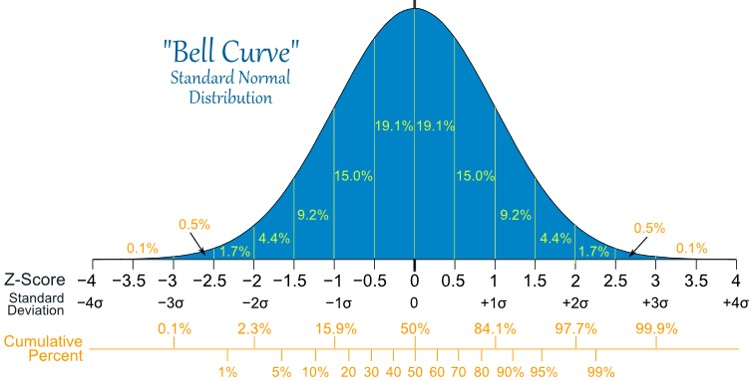
\includegraphics[width=\linewidth,keepaspectratio]{bell}
\end{center}
\end{frame}

%%%%%%%%%%%%%%%%%%%%%%%%%%%%%%%%%%%%%%%%%%%%%%%%%%%
\begin{frame}[fragile] \frametitle{Skewed Distribution}
\begin{center}
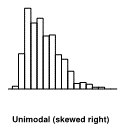
\includegraphics[width=0.3\linewidth,keepaspectratio]{skewdist}
\end{center}
\begin{itemize}
\item Skew is simply a tendency towards very high (right skew) or very low (left skew) values. 
\end{itemize}

\end{frame}

%%%%%%%%%%%%%%%%%%%%%%%%%%%%%%%%%%%%%%%%%%%%%%%%%%%
\begin{frame}[fragile] \frametitle{Exponential Distribution}
\begin{center}
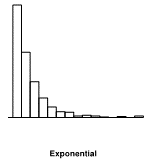
\includegraphics[width=0.3\linewidth,keepaspectratio]{expodist}
\end{center}

\begin{itemize}
\item In a feature following an exponential distribution the likelihood of occurrence of a small number of low values is very high, but sharply diminishes as values increase. 
\item Examples: number of times a person has been married; number of times a person has made an insurance claim
\end{itemize}
\end{frame}


%%%%%%%%%%%%%%%%%%%%%%%%%%%%%%%%%%%%%%%%%%%%%%%%%%%
\begin{frame}[fragile] \frametitle{Multimodal Distribution}

\begin{center}
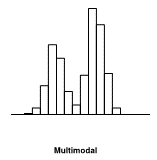
\includegraphics[width=0.3\linewidth,keepaspectratio]{mmdist}
\end{center}

\begin{itemize}
\item A feature characterized by a multimodal distribution has two or more very commonly occurring ranges of values that are clearly separated. 
\item Bi-modal distribution: two clear peaks
\item ``two normal distributions pushed together''
\item Tends to occur when a feature contains a measurement made across two distinct groups
\end{itemize}
\end{frame}



%%%%%%%%%%%%%%%%%%%%%%%%%%%%%%%%%%%%%%%%%%%%%%%%%%%%
%\begin{frame}[fragile] \frametitle{Details of Normal Distribution}
%\begin{itemize}
%\item The probability density function for the normal distribution (or Gaussian distribution) is $N(x,\mu,\sigma) = \frac{1}{\sigma \sqrt{2\pi}} e^{-\frac{(x-\mu)^2}{2\sigma^2}}$
%\item $x$ is any value
%\item $\mu$ and $\sigma$ are parameters that define the shape of the distribution
%\item the population mean and population standard deviation
%\end{itemize}
%\begin{center}
%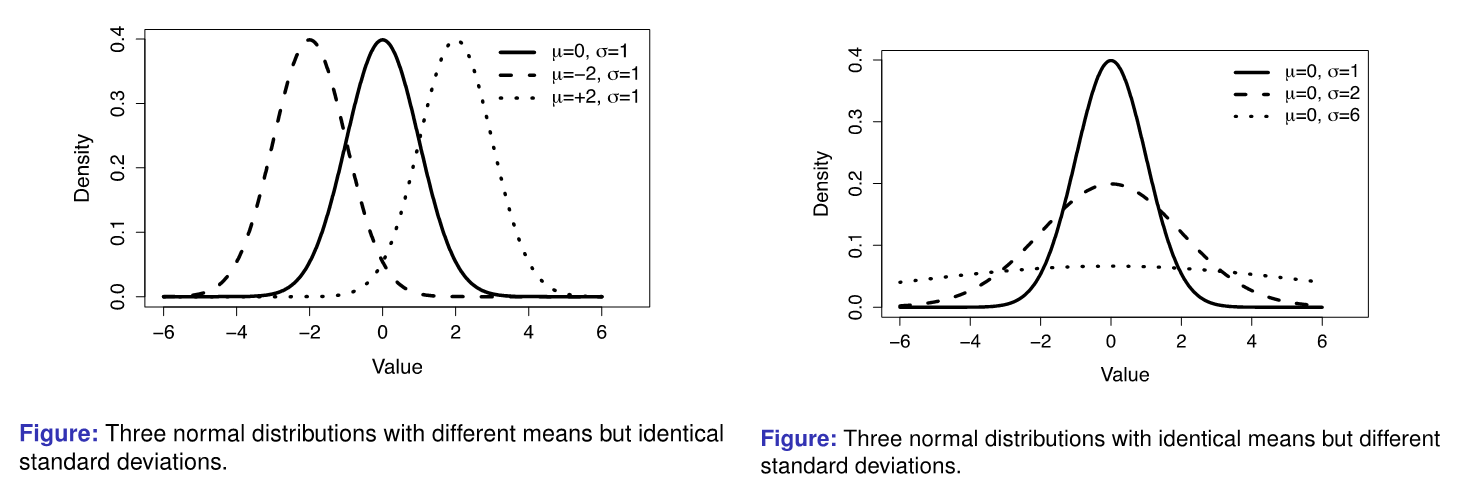
\includegraphics[width=0.8\linewidth,keepaspectratio]{stdnormdist}
%\end{center}
%\end{frame}
%





%%%%%%%%%%%%%%%%%%%%%%%%%%%%%%%%%%%%%%%%%%%%%%%%%%%%%%%%%%
\begin{frame}[fragile]\frametitle{Bi-variate  Analysis}	
\begin{itemize}
\item Finds  out  the  relationship  between  two  variables
\item Looks for association and disassociation between variables at a pre-defined significance level.
\item Most common: between Continuous  \&  Continuous: Correlation plots
\item Correlation varies between -1 and +1.
\end{itemize}
\end{frame}

%%%%%%%%%%%%%%%%%%%%%%%%%%%%%%%%%%%%%%%%%%%%%%%%%%%%%%%%%%
\begin{frame}[fragile]\frametitle{Bi-variate  Analysis}	
\begin{center}
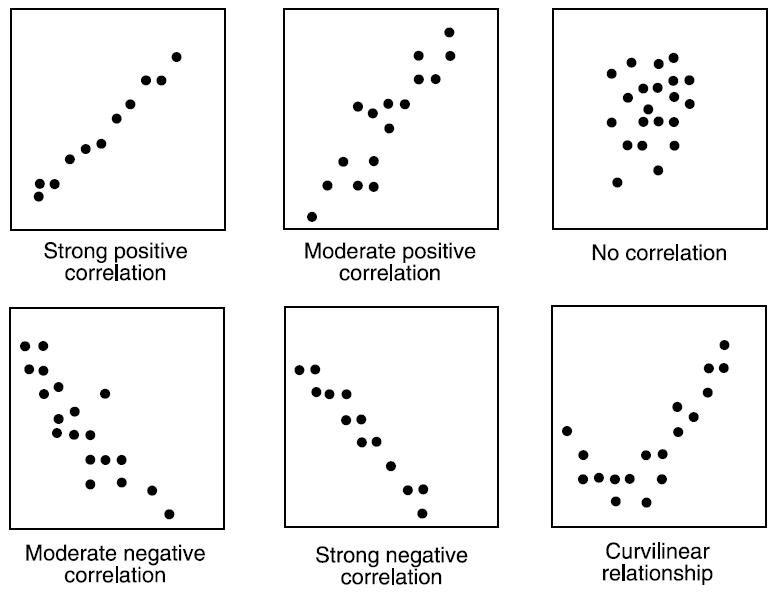
\includegraphics[width=0.8\linewidth,keepaspectratio]{eda4}
\end{center}
\end{frame}

%%%%%%%%%%%%%%%%%%%%%%%%%%%%%%%%%%%%%%%%%%%%%%%%%%%%%%%%%%
\begin{frame}[fragile]\frametitle{Bi-variate  Analysis}	
Correlation = Covariance(X,Y) / SQRT( Var(X)* Var(Y)) 	
\begin{center}
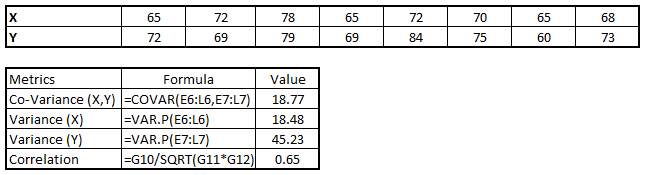
\includegraphics[width=\linewidth,keepaspectratio]{eda51}
\end{center}
\end{frame}

%%%%%%%%%%%%%%%%%%%%%%%%%%%%%%%%%%%%%%%%%%%%%%%%%%%%%%%%%%
\begin{frame}[fragile]\frametitle{Bi-variate  Analysis}
	
\begin{itemize}
\item  Chi-Square Test: Used for finding relationship between categorical variables. 
\item  Z-Test/ T-Test: Assess whether mean of two groups are statistically different from each other or not.
\item Anova: Assesses  whether  the  average  of  more  than  two  groups  is  statistically 
different.
\end{itemize}
\end{frame}

%%%%%%%%%%%%%%%%%%%%%%%%%%%%%%%%%%%%%%%%%%%%%%%%%%%%%%%%%%
\begin{frame}[fragile]\frametitle{Data collection problems}
		\begin{itemize}
			\item Missing values
			\item Outliers
			\item Inconsistent values: it often detected inconsistent data with manual
			typing or handwriting. It is important to correct the data as soon as possible.
			\item Duplicate data: Often detected when there exists two objects that 
			actually represent a single object. 
\end{itemize}
\end{frame}


%%%%%%%%%%%%%%%%%%%%%%%%%%%%%%%%%%%%%%%%%%%%%%%%%%%%%%%%%%
\begin{frame}[fragile]\frametitle{Missing Value Treatment}
Why missing values treatment is required? 
\begin{itemize}
\item   Can reduce the power / fit of a model
\item Can lead to a biased model 
\item  Can lead to wrong prediction or classification.
\end{itemize}
\end{frame}

%%%%%%%%%%%%%%%%%%%%%%%%%%%%%%%%%%%%%%%%%%%%%%%%%%%%%%%%%%
\begin{frame}[fragile]\frametitle{Missing Value Treatment}
\begin{center}
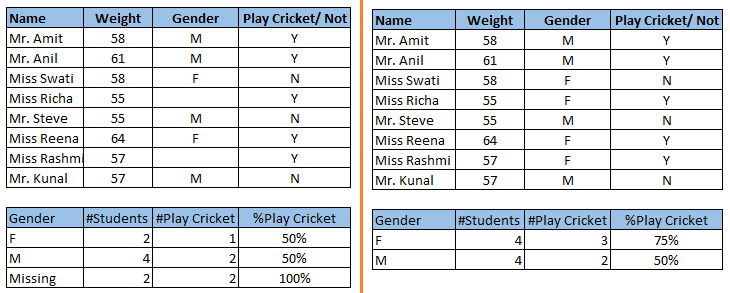
\includegraphics[width=\linewidth,keepaspectratio]{eda6}
\end{center}
\end{frame}

%%%%%%%%%%%%%%%%%%%%%%%%%%%%%%%%%%%%%%%%%%%%%%%%%%%%%%%%%%
\begin{frame}[fragile]\frametitle{Missing Value Treatment}
Why my data has missing values? 
\begin{itemize}
\item  Data Extraction: e.g text extraction failures
\item Data collection: eg Unfilled forms, transmission problems
\end{itemize}
\end{frame}

%%%%%%%%%%%%%%%%%%%%%%%%%%%%%%%%%%%%%%%%%%%%%%%%%%%%
%\begin{frame}[fragile]\frametitle{Missing Value Treatment}
%\begin{itemize}
%\item Often, values for some attributes are missing for some objects in data sets Example: individuals who decline to provide their weight in a survey
%\item Strategies:
%	\begin{itemize}
%	\item Eliminate data objects that have missing values
%	\item Eliminate data attributes if any objects are missing that value
%	\item Estimate missing values. Data set may contain similar data points
%	\item Ignore missing values. If data mining method is robust
%	\end{itemize}
%\end{itemize}
%\end{frame}


%%%%%%%%%%%%%%%%%%%%%%%%%%%%%%%%%%%%%%%%%%%%%%%%%%%%%%%%%%%
%\begin{frame}[fragile]\frametitle{Missing Value Treatment}
%\begin{center}
%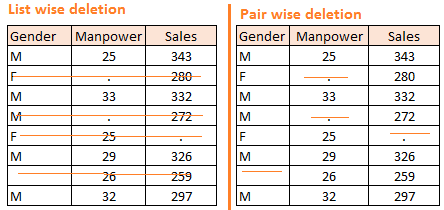
\includegraphics[width=\linewidth,keepaspectratio]{eda7}
%\end{center}
%\end{frame}

%%%%%%%%%%%%%%%%%%%%%%%%%%%%%%%%%%%%%%%%%%%%%%%%%%%%%%%%%%
\begin{frame}[fragile]\frametitle{Outliers}

		\begin{itemize}
			\item Values of an attribute that are unusual with
			respect to the typical values for that attribute. 
			\item Important to distinguish between noise and outliers.
			\item  Outliers can be legitimate data, objects or values, unlike noise, outliers may sometimes be of interest. 
\end{itemize}
\end{frame}



%%%%%%%%%%%%%%%%%%%%%%%%%%%%%%%%%%%%%%%%%%%%%%%%%%%
\begin{frame}[fragile] \frametitle{Outliers}
\begin{itemize}
\item Data objects that have characteristics that differ from most other data objects. In fraud detection, the goal is identifying these outliers
\item Value of an attribute is very unusual with respect to the typical value. Do we have a ``data error?'' or is some individual really eight foot tall?
\item Various statistical definitions for what an outliers is.
\item Outliers can be legitimate data objects or values (and may be of interest).
\end{itemize}
\end{frame}

%%%%%%%%%%%%%%%%%%%%%%%%%%%%%%%%%%%%%%%%%%%%%%%%%%%%%%%%%%
\begin{frame}[fragile] \frametitle{Outliers}
\begin{center}
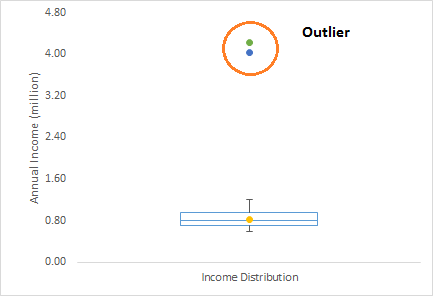
\includegraphics[width=0.8\linewidth,keepaspectratio]{eda8}
\end{center}
\end{frame}

%%%%%%%%%%%%%%%%%%%%%%%%%%%%%%%%%%%%%%%%%%%%%%%%%%%%%%%%%%
\begin{frame}[fragile] \frametitle{Outliers}
\begin{center}
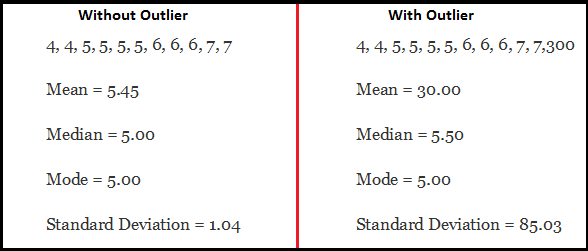
\includegraphics[width=0.8\linewidth,keepaspectratio]{eda9}
\end{center}

\begin{itemize}
\item Data set with outliers has significantly different mean and standard deviation. 
\item In the first scenario, we will say that average is 5.45. 
\item But with the outliers, average soars to 30. 
\item This would change the estimate completely. 
\end{itemize}
\end{frame}

%%%%%%%%%%%%%%%%%%%%%%%%%%%%%%%%%%%%%%%%%%%%%%%%%%%%%%%%%%%
%\begin{frame}[fragile]\frametitle{Data collection problems}
%		\begin{itemize}
%			\item {\bf Inconsistent values:} it often detected inconsistent data with manual
%			typing or handwriting. It is important to correct the data as soon as possible.
%			\item {\bf Duplicate data:} Often detected when there exists two objects that 
%			acyually represent a single object. 
%\end{itemize}
%\end{frame}


%%%%%%%%%%%%%%%%%%%%%%%%%%%%%%%%%%%%%%%%%%%%%%%%%%%
\begin{frame}[fragile] \frametitle{Inconsistent Values}
\begin{itemize}
\item Some inconsistencies are easy to detect (and fix) automatically; others are not.
\item Example:
	\begin{itemize}
	\item Data object with address, city, zip code in three separate fields
	\item But address / city is in a different zip code
	\end{itemize}
\end{itemize}
\end{frame}


%%%%%%%%%%%%%%%%%%%%%%%%%%%%%%%%%%%%%%%%%%%%%%%%%%%
\begin{frame}[fragile] \frametitle{Duplicate Values}
Example: many people receive duplicate mailings because they are in a database multiple times under slightly different names

\end{frame}


%%%%%%%%%%%%%%%%%%%%%%%%%%%%%%%%%%%%%%%%%%%%%%%%%%%
\begin{frame}[fragile] \frametitle{Case Study: Data Quality Report}
\begin{itemize}
\item A data quality report includes tabular reports that describe the characteristics of each feature in a dataset using standard statistical measures of central tendency and variation. 
\item The tabular reports are accompanied by data visualizations
	\begin{itemize}
	\item histogram for each continuous feature
	\item bar plot for each categorical feature, also generally used for continuous features with $cardinality < 10$
	\end{itemize}
\end{itemize}
\end{frame}

%%%%%%%%%%%%%%%%%%%%%%%%%%%%%%%%%%%%%%%%%%%%%%%%%%%
\begin{frame}[fragile] \frametitle{Data Quality Report}
\begin{center}
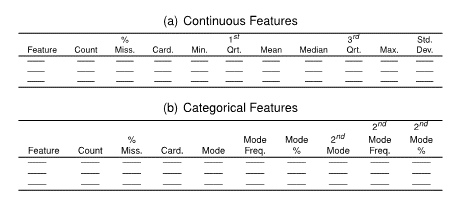
\includegraphics[width=0.6\linewidth,keepaspectratio]{dataqtable}
\end{center}
Card = Cardinality, Measures the number of distinct values present for a feature

\end{frame}


%%%%%%%%%%%%%%%%%%%%%%%%%%%%%%%%%%%%%%%%%%%%%%%%%%%
\begin{frame}[fragile] \frametitle{Case Study: Data Quality Report}

\begin{center}
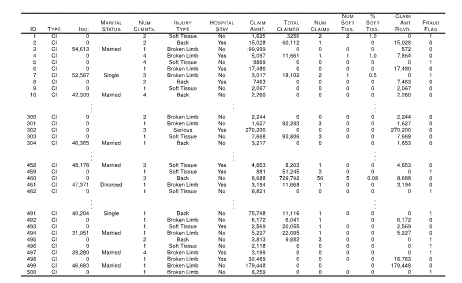
\includegraphics[width=\linewidth,keepaspectratio]{datatablecase}
\end{center}
\end{frame}

%%%%%%%%%%%%%%%%%%%%%%%%%%%%%%%%%%%%%%%%%%%%%%%%%%%
\begin{frame}[fragile] \frametitle{Case Study: Data Quality Report}

\begin{center}
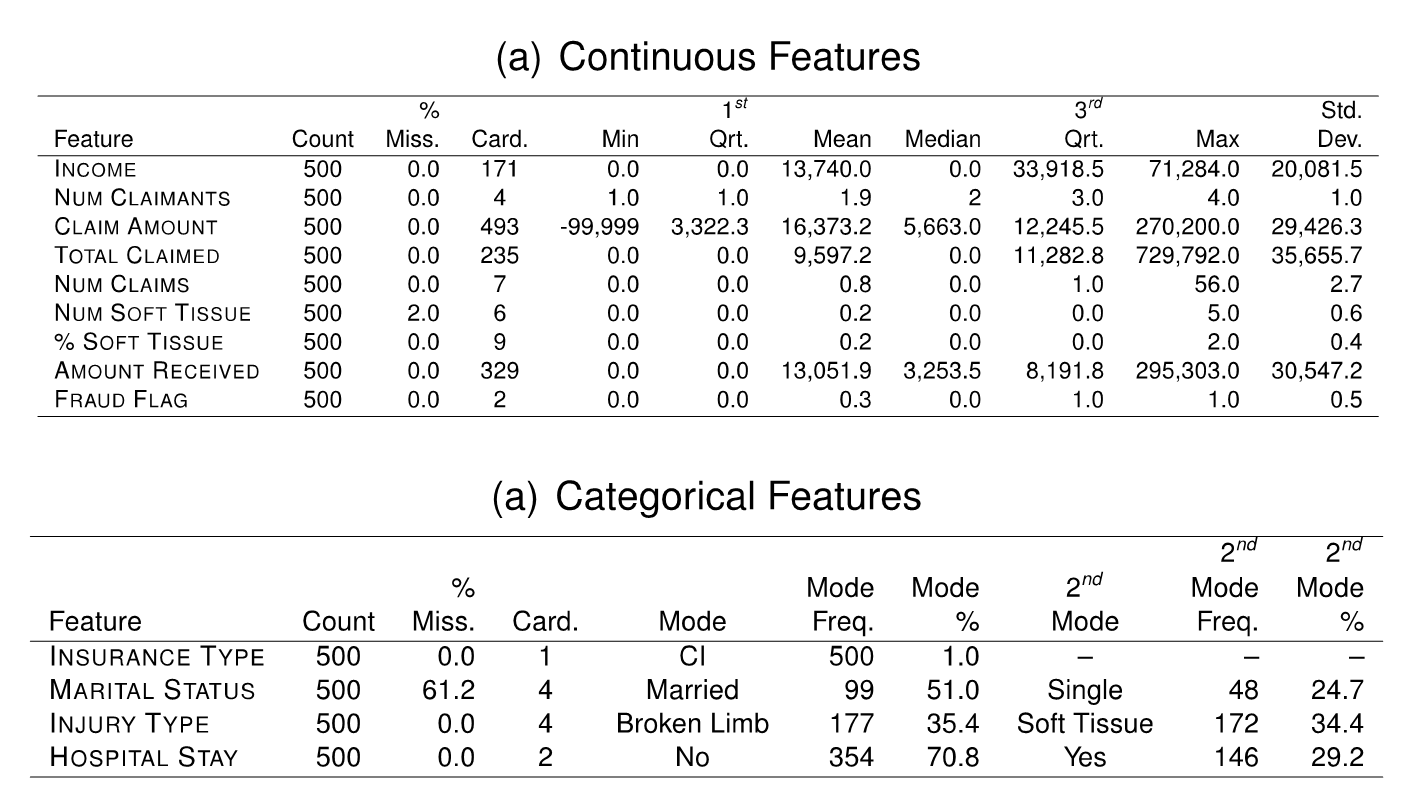
\includegraphics[width=\linewidth,keepaspectratio]{datatablecasevals}
\end{center}
\end{frame}


%%%%%%%%%%%%%%%%%%%%%%%%%%%%%%%%%%%%%%%%%%%%%%%%%%%
\begin{frame}[fragile] \frametitle{Case Study: Data Quality Report}

\begin{center}
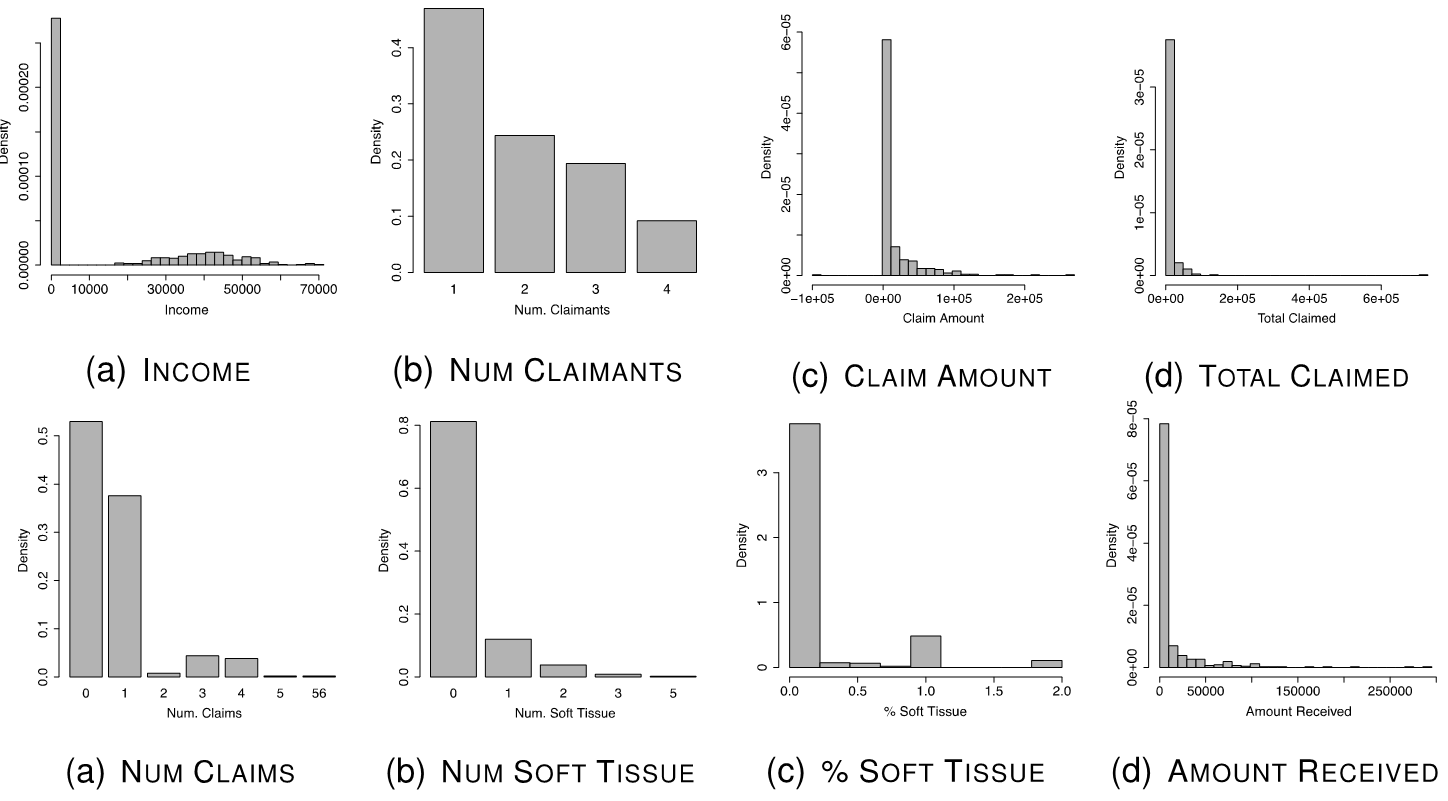
\includegraphics[width=\linewidth,keepaspectratio]{datatablecasegraphs}
\end{center}
\end{frame}

%%%%%%%%%%%%%%%%%%%%%%%%%%%%%%%%%%%%%%%%%%%%%%%%%%%
\begin{frame}[fragile] \frametitle{Case Study: Data Quality Report}

\begin{center}
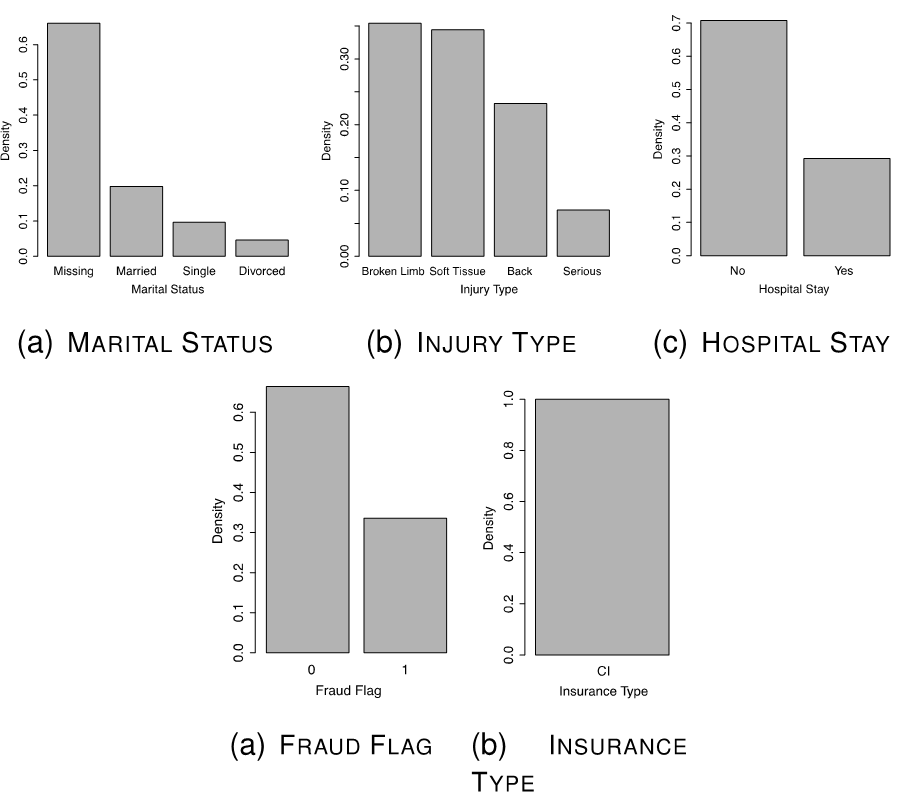
\includegraphics[width=0.7\linewidth,keepaspectratio]{datatablecasehists}
\end{center}
\end{frame}

%%%%%%%%%%%%%%%%%%%%%%%%%%%%%%%%%%%%%%%%%%%%%%%%%%%
\begin{frame}[fragile] \frametitle{Identifying Data Quality Issues}
\begin{itemize}
\item A data quality issue is loosely defined as anything unusual about the data 
\item The most common data quality issues are: 
	\begin{itemize}
	\item missing values. Rule of thumb: remove feature is more than 60\% of data is missing
	\item irregular cardinality. Cardinality of 1: everything has the same value; no useful predictive information. Continuous features will usually have a cardinality value close to the number of instances. Investigate further if cardinality seems much lower or higher than expected
	\item outliers (invalid vs. valid). Investigate using domain knowledge. Compare gap between 3rd quartile and max vs. median and 3rd quartile
	\end{itemize}
\end{itemize}
\end{frame}


%%%%%%%%%%%%%%%%%%%%%%%%%%%%%%%%%%%%%%%%%%%%%%%%%%%
\begin{frame}[fragile] \frametitle{Identifying Data Quality Issues}
\begin{itemize}
\item Data quality issues possible due to invalid data. Need to be corrected! (e.g. calculation errors, data entry errors,) 
\item Data quality issues possible due to valid data, e.g. missing data
\item Measurement error: any problem resulting from the measurement process; value recorded differs from true value to some extent
\item Data collection error
	\begin{itemize}
	\item data objects are omitted
	\item attribute values are missing for some objects
	\item inappropriately including a data object
	\end{itemize}
\end{itemize}
\end{frame}


%%%%%%%%%%%%%%%%%%%%%%%%%%%%%%%%%%%%%%%%%%%%%%%%%%%
\begin{frame}[fragile] \frametitle{Case Study}
\begin{itemize}
\item Become familiar with the central tendency and variation of each feature using the data quality report.
\item Note bar graphs and histograms (earlier slides).
\item Note number of levels and frequency of Injury Type.
\item What is the type of probability distribution for each histogram?
	\begin{itemize}
	\item Exponential Distribution: all except Income and Fraud Flag
	\item Normal Distribution: Income (except for the 0 bar)
	\item Fraud Flag: not a typical continuous feature
	\end{itemize}
\end{itemize}
\end{frame}

